% =====================================================================
% 4. Area 2: learning strategies (T13, T24: shared tasks, OF + MM)
% =====================================================================
\section{Area 2: learning strategies}\label{sec:strategies}

\subsection{Concepts}

The course distinguishes the strategies by what is re-used and which labels are needed. Transfer
learning and self-supervised learning ``both re-use knowledge'', but transfer learning is usually
trained ``with manually labelled data'', while self-supervised learning builds a more general model
``without manual labels'' by solving a \emph{pretext task} \cite{course_summary_0910}.
Self-supervised learning is a way of ``overcoming the challenges related to the scarcity of
`labelled' data'' \cite[p.~1]{soltanieh2022analysis}. A pre-trained network can be re-used in two
ways: ``fitting a linear classifier on a representation extracted from the model'' (a \emph{linear
probe} on frozen features) or ``end-to-end fine-tuning of the model'' \cite[p.~11]{radford2021learning}.
Fine-tuning usually lowers the learning rate ``to prevent catastrophic forgetting''
\cite[p.~6]{soltanieh2023indistribution}, i.e.\ to avoid ``overwriting information captured during the
initial training phase'' \cite[p.~1521]{strodthoff2021deep}. On ECG, the benefit of pre-training grows
as the labelled set shrinks \cite[p.~1524]{strodthoff2021deep}, and on 12-lead ECG ``the performance level of the supervised models at 4 folds is approximately
reached by the pretrained model trained only on two folds'' \cite[pp.~7--8]{mehari2022self}. Zero-shot classification goes one step further: no labelled
example of the target task is used. With several modalities it is possible ``thanks to a Multimodal
Correspondence'', i.e.\ embeddings of the different modalities in the same vector space
\cite{course_summary_0910}. Appendix~\ref{app:strategies} gathers these takeaways.

\subsection{Our design: a self-supervised ECG-GPT, transferred}

The ECG-GPT of area 3 (Section~\ref{sec:generative}, my block) is our self-supervised model: a small
causal Transformer trained to predict the next sample of lead II, with no diagnostic label. Its
pretext task is the GPT recipe, a ``standard language modeling objective'' \cite[p.~3]{radford2018improving}
applied to a tokenised signal; token-based autoregressive pre-training has also been applied to ECG
\cite[p.~1]{yang2025heartllm}. The pre-trained model was fixed before any transfer experiment by the
rule of the generative block (lowest validation bits per sample): the ECG-GPT with 2560 levels of
1\,\textmu V. It was pre-trained on the training folds of PTB-XL only (\generativeNRecordsTrain{}
records): a ``foundation'' model only in a very modest sense.

For the five superclasses, the network without its next-token head gives one vector per record (the
mean of its outputs over four windows of 2.5\,s), followed by dropout and a Linear layer. Three
strategies use exactly this architecture and input (tokenised lead II):
\emph{from scratch} (random weights, all trainable, learning rate $10^{-3}$), \emph{linear probe}
(pre-trained network frozen, only the head trained) and \emph{fine-tuning} (pre-trained network and
head trained together, learning rate $10^{-4}$, as in the course notebook \cite{course_nb_transfer}).
Each runs with 100\,\% and with 10\,\% of the training labels; the 10\,\% subset is drawn by patient
and is the same for the three strategies of a seed. ``10\,\%'' means 10\,\% of the \emph{labels}:
the generator had already seen the signals of every training record without labels. The reference
on the same input is the CNN trained on lead II (Section~\ref{sec:leads}).

\subsection{Results}

% Shared float (common/make_floats.py). Table: tables/transfer_main.tex
\begin{table}[htbp]
\centering
\caption[Transfer from the ECG-GPT: main results]{ECG-GPT reused for the five superclasses (lead II): the three strategies with 100\,\% and 10\,\% of the training labels (mean $\pm$ SD over seeds 42--44).}
\label{tab:transfer_main}
\small
\begin{adjustbox}{max width=\textwidth}
% Generated by src/transfer_experiments.py from results/logs/transfer_summary.json.
% Needs report/numbers.tex (alias "transfer") and booktabs.
\begin{tabular}{llrrccc}
\toprule
Labels & Strategy & Train.\ param. & Train records & Val.\ macro AUROC & Test macro AUROC & Test macro F1 \\
\midrule
100\% & From scratch & \transferParamsScratchFOneZeroZero{} & \transferNTrainScratchFOneZeroZero{} & \transferValAurocMeanScratchFOneZeroZero{} $\pm$ \transferValAurocSdScratchFOneZeroZero{} & \transferTestAurocMeanScratchFOneZeroZero{} $\pm$ \transferTestAurocSdScratchFOneZeroZero{} & \transferTestFOneMeanScratchFOneZeroZero{} $\pm$ \transferTestFOneSdScratchFOneZeroZero{} \\
100\% & Linear probe (frozen) & \transferParamsProbeFOneZeroZero{} & \transferNTrainProbeFOneZeroZero{} & \transferValAurocMeanProbeFOneZeroZero{} $\pm$ \transferValAurocSdProbeFOneZeroZero{} & \transferTestAurocMeanProbeFOneZeroZero{} $\pm$ \transferTestAurocSdProbeFOneZeroZero{} & \transferTestFOneMeanProbeFOneZeroZero{} $\pm$ \transferTestFOneSdProbeFOneZeroZero{} \\
100\% & Fine-tuning & \transferParamsFinetuneFOneZeroZero{} & \transferNTrainFinetuneFOneZeroZero{} & \transferValAurocMeanFinetuneFOneZeroZero{} $\pm$ \transferValAurocSdFinetuneFOneZeroZero{} & \transferTestAurocMeanFinetuneFOneZeroZero{} $\pm$ \transferTestAurocSdFinetuneFOneZeroZero{} & \transferTestFOneMeanFinetuneFOneZeroZero{} $\pm$ \transferTestFOneSdFinetuneFOneZeroZero{} \\
\addlinespace
10\% & From scratch & \transferParamsScratchFOneZero{} & \transferNTrainScratchFOneZero{} & \transferValAurocMeanScratchFOneZero{} $\pm$ \transferValAurocSdScratchFOneZero{} & \transferTestAurocMeanScratchFOneZero{} $\pm$ \transferTestAurocSdScratchFOneZero{} & \transferTestFOneMeanScratchFOneZero{} $\pm$ \transferTestFOneSdScratchFOneZero{} \\
10\% & Linear probe (frozen) & \transferParamsProbeFOneZero{} & \transferNTrainProbeFOneZero{} & \transferValAurocMeanProbeFOneZero{} $\pm$ \transferValAurocSdProbeFOneZero{} & \transferTestAurocMeanProbeFOneZero{} $\pm$ \transferTestAurocSdProbeFOneZero{} & \transferTestFOneMeanProbeFOneZero{} $\pm$ \transferTestFOneSdProbeFOneZero{} \\
10\% & Fine-tuning & \transferParamsFinetuneFOneZero{} & \transferNTrainFinetuneFOneZero{} & \transferValAurocMeanFinetuneFOneZero{} $\pm$ \transferValAurocSdFinetuneFOneZero{} & \transferTestAurocMeanFinetuneFOneZero{} $\pm$ \transferTestAurocSdFinetuneFOneZero{} & \transferTestFOneMeanFinetuneFOneZero{} $\pm$ \transferTestFOneSdFinetuneFOneZero{} \\
\bottomrule
\end{tabular}

\end{adjustbox}
\end{table}

% Shared float (common/make_floats.py). Figure: figures/transfer_strategies.pdf
\begin{figure}[htbp]
\centering
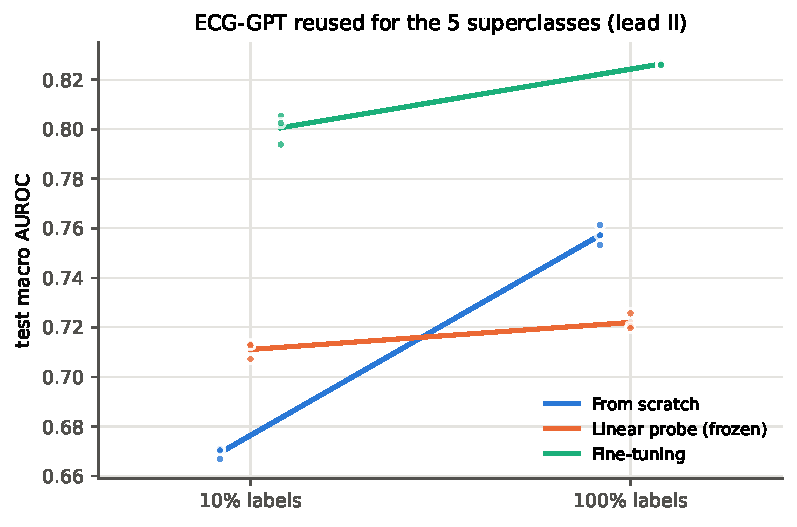
\includegraphics[width=\textwidth,height=0.42\textheight,keepaspectratio]{figures/transfer_strategies.pdf}
\caption[Transfer from the ECG-GPT: strategies and label fractions]{ECG-GPT reused for the five superclasses (lead II): test macro AUROC of training from scratch, linear probe on the frozen network and fine-tuning, with 10\,\% and 100\,\% of the training labels (dots: seeds; line: mean).}
\label{fig:transfer_strategies}
\end{figure}


\begin{enumerate}[leftmargin=1.4em,itemsep=2pt]
  \item \textbf{Pre-training pays off when the whole network is adapted.} Fine-tuning beats the same
        network from scratch by \transferTestDiffMeanFinetuneVsScratchFOneZeroZero{} with all the labels
        and by \transferTestDiffMeanFinetuneVsScratchFOneZero{} with 10\,\%, in every seed
        (Table~\ref{tab:transfer_comparisons}). The gain comes from the pre-trained weights, not from
        the smaller learning rate: with both at $10^{-4}$, fine-tuning still wins by
        \transferValDiffMeanFinetuneVsScratchLrOneEFourFOneZeroZero{} and
        \transferValDiffMeanFinetuneVsScratchLrOneEFourFOneZero{} on validation, in every seed.
  \item \textbf{Label efficiency.} Fine-tuning with 10\,\% of the labels beats training from scratch
        with all of them (\transferTestDiffMeanFinetuneFOneZeroVsScratchFOneZeroZero{}, all seeds).
        Going from 100\,\% to 10\,\% costs fine-tuning \transferTestDiffMeanFinetuneFOneZeroZeroVsFOneZero{}
        and training from scratch \transferTestDiffMeanScratchFOneZeroZeroVsFOneZero{}, as the
        literature on ECG pre-training predicts.
  \item \textbf{The frozen features are weakly diagnostic.} The linear probe is worse than training
        from scratch with all labels (\transferTestDiffMeanProbeVsScratchFOneZeroZero{}) and better
        only with 10\,\% (\transferTestDiffMeanProbeVsScratchFOneZero{}). The representation is a good
        starting point but not linearly separable by superclass. \emph{Hypothesis:} predicting the next
        sample rewards local waveform detail more than the global features that separate the classes.
  \item \textbf{The smaller learning rate was not essential.} At $10^{-3}$ fine-tuning reaches almost
        the same validation AUROC (\transferValDiffMeanLrOneEThreeVsFinetuneFOneZeroZero{} with all
        labels), only faster.
  \item \textbf{Architecture still beats pre-training here.} On the same input the CNN trained from
        scratch remains better than the fine-tuned ECG-GPT
        (\comparisonTestDiffMeanFinetuneFOneZeroZeroVsOneleadCnn{} with all labels, all seeds).
        Pre-training closes most of the gap between the ECG-GPT from scratch and the CNN, not all of
        it.
\end{enumerate}

% Shared float (common/make_floats.py). Table: tables/transfer_comparisons.tex
\begin{table}[htbp]
\centering
\caption[Transfer from the ECG-GPT: paired differences]{Paired differences in macro AUROC between transfer configurations (mean over seeds; seeds whose 95\,\% patient-bootstrap interval lies wholly above / below 0).}
\label{tab:transfer_comparisons}
\small
\begin{adjustbox}{max width=\textwidth}
% Generated by src/transfer_experiments.py from results/logs/transfer_summary.json.
% Delta = paired patient-bootstrap difference in macro AUROC, mean over seeds; better / worse = seeds whose 95% interval excludes 0.
\begin{tabular}{lcccc}
\toprule
 & \multicolumn{2}{c}{Test} & \multicolumn{2}{c}{Validation} \\
\cmidrule(lr){2-3}\cmidrule(lr){4-5}
Comparison & $\Delta$ & Seeds better / worse & $\Delta$ & Seeds better / worse \\
\midrule
Fine-tuning $-$ scratch, 100\% & \transferTestDiffMeanFinetuneVsScratchFOneZeroZero{} & \transferTestNBetterFinetuneVsScratchFOneZeroZero{} / \transferTestNWorseFinetuneVsScratchFOneZeroZero{} of \transferTestNComparedFinetuneVsScratchFOneZeroZero{} & \transferValDiffMeanFinetuneVsScratchFOneZeroZero{} & \transferValNBetterFinetuneVsScratchFOneZeroZero{} / \transferValNWorseFinetuneVsScratchFOneZeroZero{} of \transferValNComparedFinetuneVsScratchFOneZeroZero{} \\
Probe $-$ scratch, 100\% & \transferTestDiffMeanProbeVsScratchFOneZeroZero{} & \transferTestNBetterProbeVsScratchFOneZeroZero{} / \transferTestNWorseProbeVsScratchFOneZeroZero{} of \transferTestNComparedProbeVsScratchFOneZeroZero{} & \transferValDiffMeanProbeVsScratchFOneZeroZero{} & \transferValNBetterProbeVsScratchFOneZeroZero{} / \transferValNWorseProbeVsScratchFOneZeroZero{} of \transferValNComparedProbeVsScratchFOneZeroZero{} \\
Fine-tuning $-$ probe, 100\% & \transferTestDiffMeanFinetuneVsProbeFOneZeroZero{} & \transferTestNBetterFinetuneVsProbeFOneZeroZero{} / \transferTestNWorseFinetuneVsProbeFOneZeroZero{} of \transferTestNComparedFinetuneVsProbeFOneZeroZero{} & \transferValDiffMeanFinetuneVsProbeFOneZeroZero{} & \transferValNBetterFinetuneVsProbeFOneZeroZero{} / \transferValNWorseFinetuneVsProbeFOneZeroZero{} of \transferValNComparedFinetuneVsProbeFOneZeroZero{} \\
Fine-tuning $-$ scratch, 10\% & \transferTestDiffMeanFinetuneVsScratchFOneZero{} & \transferTestNBetterFinetuneVsScratchFOneZero{} / \transferTestNWorseFinetuneVsScratchFOneZero{} of \transferTestNComparedFinetuneVsScratchFOneZero{} & \transferValDiffMeanFinetuneVsScratchFOneZero{} & \transferValNBetterFinetuneVsScratchFOneZero{} / \transferValNWorseFinetuneVsScratchFOneZero{} of \transferValNComparedFinetuneVsScratchFOneZero{} \\
Probe $-$ scratch, 10\% & \transferTestDiffMeanProbeVsScratchFOneZero{} & \transferTestNBetterProbeVsScratchFOneZero{} / \transferTestNWorseProbeVsScratchFOneZero{} of \transferTestNComparedProbeVsScratchFOneZero{} & \transferValDiffMeanProbeVsScratchFOneZero{} & \transferValNBetterProbeVsScratchFOneZero{} / \transferValNWorseProbeVsScratchFOneZero{} of \transferValNComparedProbeVsScratchFOneZero{} \\
Fine-tuning $-$ probe, 10\% & \transferTestDiffMeanFinetuneVsProbeFOneZero{} & \transferTestNBetterFinetuneVsProbeFOneZero{} / \transferTestNWorseFinetuneVsProbeFOneZero{} of \transferTestNComparedFinetuneVsProbeFOneZero{} & \transferValDiffMeanFinetuneVsProbeFOneZero{} & \transferValNBetterFinetuneVsProbeFOneZero{} / \transferValNWorseFinetuneVsProbeFOneZero{} of \transferValNComparedFinetuneVsProbeFOneZero{} \\
From scratch: 100\% $-$ 10\% labels & \transferTestDiffMeanScratchFOneZeroZeroVsFOneZero{} & \transferTestNBetterScratchFOneZeroZeroVsFOneZero{} / \transferTestNWorseScratchFOneZeroZeroVsFOneZero{} of \transferTestNComparedScratchFOneZeroZeroVsFOneZero{} & \transferValDiffMeanScratchFOneZeroZeroVsFOneZero{} & \transferValNBetterScratchFOneZeroZeroVsFOneZero{} / \transferValNWorseScratchFOneZeroZeroVsFOneZero{} of \transferValNComparedScratchFOneZeroZeroVsFOneZero{} \\
Linear probe (frozen): 100\% $-$ 10\% labels & \transferTestDiffMeanProbeFOneZeroZeroVsFOneZero{} & \transferTestNBetterProbeFOneZeroZeroVsFOneZero{} / \transferTestNWorseProbeFOneZeroZeroVsFOneZero{} of \transferTestNComparedProbeFOneZeroZeroVsFOneZero{} & \transferValDiffMeanProbeFOneZeroZeroVsFOneZero{} & \transferValNBetterProbeFOneZeroZeroVsFOneZero{} / \transferValNWorseProbeFOneZeroZeroVsFOneZero{} of \transferValNComparedProbeFOneZeroZeroVsFOneZero{} \\
Fine-tuning: 100\% $-$ 10\% labels & \transferTestDiffMeanFinetuneFOneZeroZeroVsFOneZero{} & \transferTestNBetterFinetuneFOneZeroZeroVsFOneZero{} / \transferTestNWorseFinetuneFOneZeroZeroVsFOneZero{} of \transferTestNComparedFinetuneFOneZeroZeroVsFOneZero{} & \transferValDiffMeanFinetuneFOneZeroZeroVsFOneZero{} & \transferValNBetterFinetuneFOneZeroZeroVsFOneZero{} / \transferValNWorseFinetuneFOneZeroZeroVsFOneZero{} of \transferValNComparedFinetuneFOneZeroZeroVsFOneZero{} \\
Fine-tuning 10\% $-$ scratch 100\% & \transferTestDiffMeanFinetuneFOneZeroVsScratchFOneZeroZero{} & \transferTestNBetterFinetuneFOneZeroVsScratchFOneZeroZero{} / \transferTestNWorseFinetuneFOneZeroVsScratchFOneZeroZero{} of \transferTestNComparedFinetuneFOneZeroVsScratchFOneZeroZero{} & \transferValDiffMeanFinetuneFOneZeroVsScratchFOneZeroZero{} & \transferValNBetterFinetuneFOneZeroVsScratchFOneZeroZero{} / \transferValNWorseFinetuneFOneZeroVsScratchFOneZeroZero{} of \transferValNComparedFinetuneFOneZeroVsScratchFOneZeroZero{} \\
Fine-tuning lr 1e-3 $-$ lr 1e-4, 100\% & --- & --- & \transferValDiffMeanLrOneEThreeVsFinetuneFOneZeroZero{} & \transferValNBetterLrOneEThreeVsFinetuneFOneZeroZero{} / \transferValNWorseLrOneEThreeVsFinetuneFOneZeroZero{} of \transferValNComparedLrOneEThreeVsFinetuneFOneZeroZero{} \\
Scratch lr 1e-4 $-$ lr 1e-3, 100\% & --- & --- & \transferValDiffMeanLrOneEFourVsScratchFOneZeroZero{} & \transferValNBetterLrOneEFourVsScratchFOneZeroZero{} / \transferValNWorseLrOneEFourVsScratchFOneZeroZero{} of \transferValNComparedLrOneEFourVsScratchFOneZeroZero{} \\
Fine-tuning $-$ scratch, both lr 1e-4, 100\% & --- & --- & \transferValDiffMeanFinetuneVsScratchLrOneEFourFOneZeroZero{} & \transferValNBetterFinetuneVsScratchLrOneEFourFOneZeroZero{} / \transferValNWorseFinetuneVsScratchLrOneEFourFOneZeroZero{} of \transferValNComparedFinetuneVsScratchLrOneEFourFOneZeroZero{} \\
Fine-tuning lr 1e-3 $-$ lr 1e-4, 10\% & --- & --- & \transferValDiffMeanLrOneEThreeVsFinetuneFOneZero{} & \transferValNBetterLrOneEThreeVsFinetuneFOneZero{} / \transferValNWorseLrOneEThreeVsFinetuneFOneZero{} of \transferValNComparedLrOneEThreeVsFinetuneFOneZero{} \\
Scratch lr 1e-4 $-$ lr 1e-3, 10\% & --- & --- & \transferValDiffMeanLrOneEFourVsScratchFOneZero{} & \transferValNBetterLrOneEFourVsScratchFOneZero{} / \transferValNWorseLrOneEFourVsScratchFOneZero{} of \transferValNComparedLrOneEFourVsScratchFOneZero{} \\
Fine-tuning $-$ scratch, both lr 1e-4, 10\% & --- & --- & \transferValDiffMeanFinetuneVsScratchLrOneEFourFOneZero{} & \transferValNBetterFinetuneVsScratchLrOneEFourFOneZero{} / \transferValNWorseFinetuneVsScratchLrOneEFourFOneZero{} of \transferValNComparedFinetuneVsScratchLrOneEFourFOneZero{} \\
Probe base $-$ probe selected, 100\% & --- & --- & \transferValDiffMeanProbeBaseVsProbeFOneZeroZero{} & \transferValNBetterProbeBaseVsProbeFOneZeroZero{} / \transferValNWorseProbeBaseVsProbeFOneZeroZero{} of \transferValNComparedProbeBaseVsProbeFOneZeroZero{} \\
Probe base $-$ probe selected, 10\% & --- & --- & \transferValDiffMeanProbeBaseVsProbeFOneZero{} & \transferValNBetterProbeBaseVsProbeFOneZero{} / \transferValNWorseProbeBaseVsProbeFOneZero{} of \transferValNComparedProbeBaseVsProbeFOneZero{} \\
Probe lstm $-$ probe selected, 100\% & --- & --- & \transferValDiffMeanProbeLstmVsProbeFOneZeroZero{} & \transferValNBetterProbeLstmVsProbeFOneZeroZero{} / \transferValNWorseProbeLstmVsProbeFOneZeroZero{} of \transferValNComparedProbeLstmVsProbeFOneZeroZero{} \\
Probe lstm $-$ probe selected, 10\% & --- & --- & \transferValDiffMeanProbeLstmVsProbeFOneZero{} & \transferValNBetterProbeLstmVsProbeFOneZero{} / \transferValNWorseProbeLstmVsProbeFOneZero{} of \transferValNComparedProbeLstmVsProbeFOneZero{} \\
Probe ctx100 $-$ probe selected, 100\% & --- & --- & \transferValDiffMeanProbeCtxOneZeroZeroVsProbeFOneZeroZero{} & \transferValNBetterProbeCtxOneZeroZeroVsProbeFOneZeroZero{} / \transferValNWorseProbeCtxOneZeroZeroVsProbeFOneZeroZero{} of \transferValNComparedProbeCtxOneZeroZeroVsProbeFOneZeroZero{} \\
Probe ctx100 $-$ probe selected, 10\% & --- & --- & \transferValDiffMeanProbeCtxOneZeroZeroVsProbeFOneZero{} & \transferValNBetterProbeCtxOneZeroZeroVsProbeFOneZero{} / \transferValNWorseProbeCtxOneZeroZeroVsProbeFOneZero{} of \transferValNComparedProbeCtxOneZeroZeroVsProbeFOneZero{} \\
Probe vocab64 $-$ probe selected, 100\% & --- & --- & \transferValDiffMeanProbeVocabSixFourVsProbeFOneZeroZero{} & \transferValNBetterProbeVocabSixFourVsProbeFOneZeroZero{} / \transferValNWorseProbeVocabSixFourVsProbeFOneZeroZero{} of \transferValNComparedProbeVocabSixFourVsProbeFOneZeroZero{} \\
Probe vocab64 $-$ probe selected, 10\% & --- & --- & \transferValDiffMeanProbeVocabSixFourVsProbeFOneZero{} & \transferValNBetterProbeVocabSixFourVsProbeFOneZero{} / \transferValNWorseProbeVocabSixFourVsProbeFOneZero{} of \transferValNComparedProbeVocabSixFourVsProbeFOneZero{} \\
Probe no\_pos $-$ probe selected, 100\% & --- & --- & \transferValDiffMeanProbeNoPosVsProbeFOneZeroZero{} & \transferValNBetterProbeNoPosVsProbeFOneZeroZero{} / \transferValNWorseProbeNoPosVsProbeFOneZeroZero{} of \transferValNComparedProbeNoPosVsProbeFOneZeroZero{} \\
Probe no\_pos $-$ probe selected, 10\% & --- & --- & \transferValDiffMeanProbeNoPosVsProbeFOneZero{} & \transferValNBetterProbeNoPosVsProbeFOneZero{} / \transferValNWorseProbeNoPosVsProbeFOneZero{} of \transferValNComparedProbeNoPosVsProbeFOneZero{} \\
Probe ctx500 $-$ probe selected, 100\% & --- & --- & \transferValDiffMeanProbeCtxFiveZeroZeroVsProbeFOneZeroZero{} & \transferValNBetterProbeCtxFiveZeroZeroVsProbeFOneZeroZero{} / \transferValNWorseProbeCtxFiveZeroZeroVsProbeFOneZeroZero{} of \transferValNComparedProbeCtxFiveZeroZeroVsProbeFOneZeroZero{} \\
Probe ctx500 $-$ probe selected, 10\% & --- & --- & \transferValDiffMeanProbeCtxFiveZeroZeroVsProbeFOneZero{} & \transferValNBetterProbeCtxFiveZeroZeroVsProbeFOneZero{} / \transferValNWorseProbeCtxFiveZeroZeroVsProbeFOneZero{} of \transferValNComparedProbeCtxFiveZeroZeroVsProbeFOneZero{} \\
\bottomrule
\end{tabular}

\end{adjustbox}
\end{table}


\paragraph{A better generator does not give better features.} We also trained the same linear probe
on every other generator of area 3 (Figure~\ref{fig:transfer_probe_study}). All of them give better
frozen features than the selected one, chosen for being the best density model; the correlation
between bits per sample and probe AUROC is positive (Spearman \transferProbeSpearmanFOneZeroZero{}
with all labels, \transferProbeSpearmanFOneZero{} with 10\,\%), i.e.\ worse generators tend to give
\emph{better} features. The LSTM generator gives the best probe with all labels
(\transferValAurocMeanProbeLstmFOneZeroZero{} against \transferValAurocMeanProbeFOneZeroZero{}).
\emph{Hypotheses, not tested:} with 2560 levels the embedding spends its capacity on fine amplitude
detail; the LSTM state summarises the window more than a mean of causal outputs does. The selection
rule was reasonable and fixed in advance, but in hindsight it was not the best rule for transfer. We
report this as a finding and did not change the main experiment after the fact.

% Shared float (common/make_floats.py). Figure: figures/transfer_probe_study.pdf
\begin{figure}[htbp]
\centering
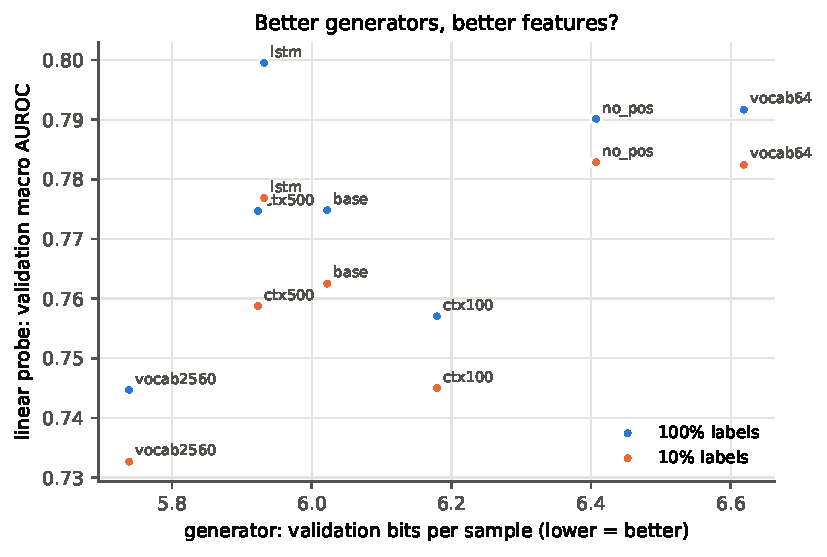
\includegraphics[width=\textwidth,height=0.42\textheight,keepaspectratio]{figures/transfer_probe_study.pdf}
\caption[Probe study: generator quality against feature quality]{Probe study: validation bits per sample of each generator of the generative block against the validation macro AUROC of a linear probe on its frozen features (mean over seeds), with 100\,\% and 10\,\% of the labels.}
\label{fig:transfer_probe_study}
\end{figure}


\paragraph{Limitations.} The probe with 10\,\% of the labels reached its best epoch near the 50-epoch
limit (on average epoch \intval{\transferBestEpochMeanProbeFOneZero}), so it was limited by the
budget. Early stopping and the F1 thresholds of the 10\,\% runs used the whole validation fold, which
has about as many labelled records as the 10\,\% training subset; a truly label-scarce setting would
also have a small validation set.

\subsection{Zero-shot learning with CLIP}

Our ECG-GPT has no text side, so it can be transferred but cannot classify zero-shot. To study
zero-shot we used CLIP, the model of the course notebook \cite{course_nb_clip}, trained on ``400
million (image, text) pairs collected form a variety of publicly available sources on the Internet''
\cite[p.~3]{radford2021learning}. It classifies by computing the cosine similarity between the image
and each class sentence, ``scaled by a temperature parameter $\tau$, and normalized into a probability
distribution via a softmax'' \cite[p.~6]{radford2021learning}. Nothing was trained or tuned; the
sentences were fixed before the run.

% Shared float (common/make_floats.py). Table: tables/zeroshot.tex
\begin{table}[htbp]
\centering
\caption[Zero-shot CLIP]{Zero-shot CLIP ViT-B/32: CIFAR-100 (where zero-shot should work) and PTB-XL lead II images (95\,\% bootstrap intervals; patients as the unit on PTB-XL).}
\label{tab:zeroshot}
\small
\begin{adjustbox}{max width=\textwidth}
% Generated by src/zero_shot.py from results/logs/zeroshot.json.
% Needs report/numbers.tex (alias "zeroshot") and booktabs.
\begin{tabular}{llc}
\toprule
Data & Measure & Value [95\% CI] \\
\midrule
CIFAR-100 & top-1 accuracy, ``This is a photo of a \{label\}'' & \zeroshotCifarTopOneNotebook{} [\zeroshotCifarTopOneLoNotebook{}, \zeroshotCifarTopOneHiNotebook{}] \\
CIFAR-100 & top-5 accuracy, ``This is a photo of a \{label\}'' & \zeroshotCifarTopFiveNotebook{} [\zeroshotCifarTopFiveLoNotebook{}, \zeroshotCifarTopFiveHiNotebook{}] \\
CIFAR-100 & top-1 accuracy, bare label & \zeroshotCifarTopOneLabel{} [\zeroshotCifarTopOneLoLabel{}, \zeroshotCifarTopOneHiLabel{}] \\
CIFAR-100 & top-5 accuracy, bare label & \zeroshotCifarTopFiveLabel{} [\zeroshotCifarTopFiveLoLabel{}, \zeroshotCifarTopFiveHiLabel{}] \\
CIFAR-100 & chance (top-1) & \zeroshotCifarChanceTopOne{} \\
\midrule
PTB-XL lead II & images seen as ``an electrocardiogram'' & \zeroshotFracModalityEcgTest{} \\
PTB-XL lead II & macro AUROC, validation & \zeroshotValMacroAuroc{} [\zeroshotValMacroAurocLo{}, \zeroshotValMacroAurocHi{}] \\
PTB-XL lead II & macro AUROC, test & \zeroshotTestMacroAuroc{} [\zeroshotTestMacroAurocLo{}, \zeroshotTestMacroAurocHi{}] \\
PTB-XL lead II & AUROC NORM, test & \zeroshotTestAurocNORM{} [\zeroshotTestAurocNORMLo{}, \zeroshotTestAurocNORMHi{}] \\
PTB-XL lead II & AUROC MI, test & \zeroshotTestAurocMI{} [\zeroshotTestAurocMILo{}, \zeroshotTestAurocMIHi{}] \\
PTB-XL lead II & AUROC STTC, test & \zeroshotTestAurocSTTC{} [\zeroshotTestAurocSTTCLo{}, \zeroshotTestAurocSTTCHi{}] \\
PTB-XL lead II & AUROC CD, test & \zeroshotTestAurocCD{} [\zeroshotTestAurocCDLo{}, \zeroshotTestAurocCDHi{}] \\
PTB-XL lead II & AUROC HYP, test & \zeroshotTestAurocHYP{} [\zeroshotTestAurocHYPLo{}, \zeroshotTestAurocHYPHi{}] \\
\bottomrule
\end{tabular}

\end{adjustbox}
\end{table}

% Shared float (common/make_floats.py). Figure: figures/zeroshot_examples.pdf
\begin{figure}[htbp]
\centering
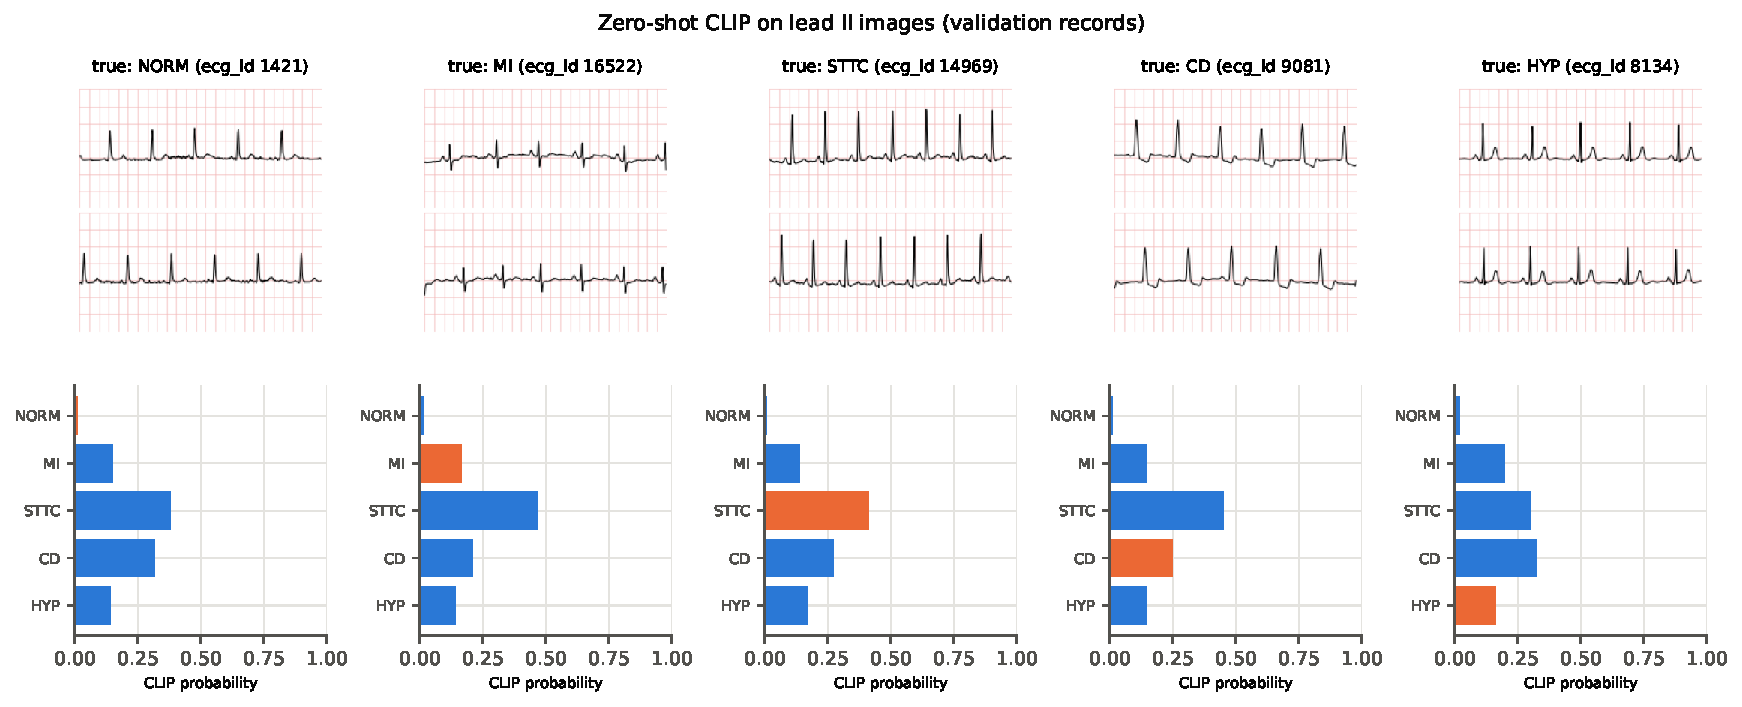
\includegraphics[width=\textwidth,height=0.42\textheight,keepaspectratio]{figures/zeroshot_examples.pdf}
\caption[Zero-shot CLIP: examples]{Zero-shot CLIP on lead II drawn as an image (one validation record per superclass): the image given to CLIP and the probability of each class sentence; orange: the true class.}
\label{fig:zeroshot_examples}
\end{figure}


On CIFAR-100, where zero-shot is expected to work, CLIP picks the right class among
\zeroshotCifarNClasses{} for a share \zeroshotCifarTopOneNotebook{} of the test images (chance
\zeroshotCifarChanceTopOne{}), and the notebook's sentence ``This is a photo of a \{label\}'' helps
over the bare label. On ECG images drawn from lead II, CLIP recognises the modality (the sentence
``an electrocardiogram'' is the closest of six for \zeroshotFracModalityEcgTestPct{} of the test
records) but not the diagnosis: macro AUROC \zeroshotTestMacroAuroc{}, barely above chance and below
the trivial model (\comparisonTestDiffMeanZeroshotVsTrivial{}). The ST-T sentence wins for
\zeroshotFracTopSTTCTestPct{} of the records whatever their class, and MI is ranked against the truth
(AUROC \zeroshotTestAurocMI{}). The source states what CLIP was trained on, not whether ECG traces
paired with diagnoses are among those pairs; that they are too rare to tie the trace to the diagnosis
is our \emph{hypothesis}. Zero-shot therefore needs a shared space that covers the task, not only the
modality.
